% ==============================================================================
%
%                             Image Processing
%
% ==============================================================================
\chapter{Image Processing}  \label{chapt:image_processing}
The Wallis as a local contrast enhancement filter is implemented as an IP core. First the concept of the algorithm is shown and then the implementation of the filter in Vivado HLS using C/C++ code is documented. The simplifications and optimizations of the algorithm with Vivado HLS are explained in chapter \ref{ch:ip:hls_opt}. \\
During the work on the project it has been discovered that the throughput does not reach the maximum and therefore will not lead to the optimum solution (see chapter \ref{chapt:ver_bench}). This is why a second implementation of the Wallis filter was made using VHDL. This second implementation is explained in chapter \ref{ch:ip:imp_vhdl} with a concept of the VHDL design.

\section{Concept} \label{ch:ip:concept}
Figure \ref{fig:concept} shows the concept of the C/C++ code programmed in Vivado HLS. First, the local mean and variance values must be calculated so that the Wallis filter can be applied with the given parameters to the pixel $I(x,y)$. The calculation of mean and variance is explained in chapter \ref{ch:ip:mean_var}. The calculated pixel is $I'(x,y)$. \\
The sequence of the code is shown in figure \ref{fig:sequence}. It consists of an initialization and an iteration. During the initialization, the complete neighborhood (here as an example 3x3) is read and the central pixel of the neighborhood is calculated. To calculate the next pixel, only one new column (gray marked) is read and the old column (hatched line) can be dismissed. This step is the so called iteration.\\
The operation is row based. This means that each new output row of the image requires the initialization procedure.

\begin{figure}[tb!]
    \centering
    \begin{adjustbox}{max width=\textwidth}
        % \tikzsetnextfilename{system-overview}

\tikzset{%
  do path picture/.style={%
    path picture={%
      \pgfpointdiff{\pgfpointanchor{path picture bounding box}{south west}}%
        {\pgfpointanchor{path picture bounding box}{north east}}%
      \pgfgetlastxy\x\y%
      \tikzset{x=\x/2,y=\y/2}%
      #1
    }
  },
  sin wave/.style={do path picture={    
    \draw [line cap=round] (-3/4,0)
      sin (-3/8,1/2) cos (0,0) sin (3/8,-1/2) cos (3/4,0);
  }},
  cross/.style={do path picture={    
    \draw [line cap=round] (-1,-1) -- (1,1) (-1,1) -- (1,-1);
  }},
  plus/.style={do path picture={    
    \draw [line cap=round] (-3/4,0) -- (3/4,0) (0,-3/4) -- (0,3/4);
  }}
}

\begin{tikzpicture}[
    rounded corners=0mm, 
]
    %coordinates
    \coordinate (wallis)    at (13,-4.135);
    \coordinate (sum0)      at (3,-1.5);
    \coordinate (sum1)      at (3,-4);
    \coordinate (plus0)     at (1.5,-1.25);
    \coordinate (plus1)     at (1.5,-3.75);
    \coordinate (plus2)     at (6.5,-3.75);
    \coordinate (square0)   at (0,-3.95);
    \coordinate (square1)   at (6.5,-2.75);
    \coordinate (divide0)   at (5,-1.5);
    \coordinate (divide1)   at (5,-4);

    %nodes
    \node[draw, fill=white, minimum width=4.04cm, minimum height=4.04cm, anchor=south, align=center, label={[xshift=-1cm, yshift=0cm]Wallis Filter}] (wallis) at (wallis) {$I'(x,y)$};
    \node[draw, fill=white, minimum width=1cm, minimum height=1cm, anchor=south, align=center] (sum0) at (sum0) {\huge $\Sigma$};
    \node[draw, fill=white, minimum width=1cm, minimum height=1cm, anchor=south, align=center] (sum1) at (sum1) {\huge $\Sigma$};
    \node [circle, draw, minimum width=0.5cm, minimum height=0.5cm, anchor=south, align=center, plus] (plus0) at (plus0) {};
    \node [circle, draw, minimum width=0.5cm, minimum height=0.5cm, anchor=south, align=center, plus] (plus1) at (plus1) {};
    \node [circle, draw, minimum width=0.5cm, minimum height=0.5cm, anchor=south, align=center, plus] (plus2) at (plus2) {};
    \node [circle, draw, minimum width=0.5cm, minimum height=0.5cm, anchor=south, align=center] (divide0) at (divide0) {$\frac{1}{441}$};
    \node [circle, draw, minimum width=0.5cm, minimum height=0.5cm, anchor=south, align=center] (divide1) at (divide1) {$\frac{1}{441}$};
    \node [circle, draw, minimum width=0.5cm, minimum height=0.5cm, anchor=south, align=center] (square0) at (square0) {$()^2$};
    \node [circle, draw, minimum width=0.5cm, minimum height=0.5cm, anchor=south, align=center] (square1) at (square1) {$()^2$};


    \node[draw,fit={($(sum0.north)+(0,8pt)$) (sum1) (plus0) (plus1) (plus2) (square0) (square1) (divide0) (divide1)}] {}; 
    \node[above,xshift=0.85cm,yshift=0cm] {Mean \& Variance};

    %path
    \path[draw,-{Latex[length=2.5mm]}] (-1.75,-2) node[above,xshift=0.4cm,yshift=0cm]{pixel} -- ++(1.75,0) |- (plus0.west);
    \path[draw,-{Latex[length=2.5mm]}] (-1.75,-2) -- ++(1.75,0) -- (square0);

    %mean
    \path[draw,-{Latex[length=2.5mm]}] (plus0) -- (sum0);
    \path[draw,-{Latex[length=2.5mm]}] (sum0) -- (divide0);
    \path[draw,-{Latex[length=2.5mm]}] (divide0) -| (square1);
    \path[draw,-{Latex[length=2.5mm]}] (sum0.north) |- ++(-0.75,0.25) -| node[above,xshift=-0.25cm,yshift=-0.65cm] {$-$} (plus0.north);

    %variance
    \path[draw,-{Latex[length=2.5mm]}] (square0) -- (plus1);
    \path[draw,-{Latex[length=2.5mm]}] (plus1) -- (sum1);
    \path[draw,-{Latex[length=2.5mm]}] (sum1.north) |- ++(-0.75,0.25) -| node[above,xshift=-0.25cm,yshift=-0.65cm] {$-$} (plus1.north);
    %\path[draw,-{Latex[length=2.5mm]}] (sum1.north) |- node[above,xshift=0cm,yshift=0cm] {$-$} (plus1.east);
    %\path[draw,-{Latex[length=2.5mm]}] (plus1.south) |- (sum1.157);
    \path[draw,-{Latex[length=2.5mm]}] (sum1) -- (divide1);
    \path[draw,-{Latex[length=2.5mm]}] (divide1) -- (plus2);
    \path[draw,-{Latex[length=2.5mm]}] (square1) -- node[above,xshift=-0.25cm,yshift=-0.4cm] {$-$} (plus2);

    %wallis
    \path[draw,-{Latex[length=2.5mm]}] (divide0) -- node[above,xshift=2.2cm,yshift=0cm]{$\mu_n$} (wallis.151);
    \path[draw,-{Latex[length=2.5mm]}] (plus2) -- ++(1,0) |- node[above,xshift=2.95cm,yshift=0cm]{$\sigma_{n}^{2}$} (wallis.171);
    \path[draw,-{Latex[length=2.5mm]}] (9,-2.5) -- node[above,xshift=0.16cm,yshift=0cm]{$I(x,y)$} (wallis.191);
    \path[draw,-{Latex[length=2.5mm]}] (9,-3.325) -- node[above,xshift=-0.15cm,yshift=0cm]{parameter} (wallis.211);
    \path[draw,-{Latex[length=2.5mm]}] (wallis) -- node[above,xshift=-0.2cm,yshift=0cm]{$I'(x,y)$} (16.75,-2.11);




\end{tikzpicture}
    \end{adjustbox}
    \caption{Concept of the Wallis filter implementation}
    \label{fig:concept}
\end{figure}

\begin{figure}[tb!]
    \centering
    \begin{adjustbox}{max width=\textwidth}
        % \tikzsetnextfilename{system-overview}

\begin{tikzpicture}[
    rounded corners=0mm, 
]
    %%%%%%%%%%%%%%%%%%%%%%%%%%%%%
    %%% Second Row %%%
    %%%%%%%%%%%%%%%%%%%%%%%%%%%%%
    \begin{scope}
        % Grid
        \draw (0, 0) grid (8, 6);

        % Window Size
        \fill[gray!30, draw=black] (0,2) rectangle (1,3);
        \fill[gray!30, draw=black] (1,2) rectangle (2,3);
        \fill[gray!30, draw=black] (2,2) rectangle (3,3);
        \fill[gray!30, draw=black] (0,3) rectangle (1,4);
        \fill[gray!30, draw=black] (1,3) rectangle (2,4);
        \fill[gray!30, draw=black] (2,3) rectangle (3,4);
        \fill[gray!30, draw=black] (0,4) rectangle (1,5);
        \fill[gray!30, draw=black] (1,4) rectangle (2,5);
        \fill[gray!30, draw=black] (2,4) rectangle (3,5);
        \draw[very thick] (0,2) rectangle (3,5);

        % Center Pixel
        \draw[black,line width=0.5mm] (1,3) rectangle (2,4);

        % Text
        \node[anchor=center] at (4, 6.5) {\huge Initialization};
    \end{scope}

    \begin{scope}[xshift=9.5cm]
        % Grid
        \draw (0, 0) grid (8, 6);

        %Coloring
        \draw[pattern=north east lines, pattern color=gray] (0,2) rectangle (1,3);
        \draw[pattern=north east lines, pattern color=gray] (0,3) rectangle (1,4);
        \draw[pattern=north east lines, pattern color=gray] (0,4) rectangle (1,5);
        \fill[gray!30, draw=black] (3,2) rectangle (4,3);
        \fill[gray!30, draw=black] (3,3) rectangle (4,4);
        \fill[gray!30, draw=black] (3,4) rectangle (4,5);

        % Window Size
        \draw[very thick] (1,2) rectangle (4,5);

        % Center Pixel
        \draw[black,line width=0.5mm] (2,3) rectangle (3,4);

        % Text
        \node[anchor=center] at (4, 6.5) {\huge Iteration};
    \end{scope}

    \begin{scope}[xshift=19cm]
        % Grid
        \draw (0, 0) grid (8, 6);

        %Coloring
        \draw[pattern=north east lines, pattern color=gray] (1,2) rectangle (2,3);
        \draw[pattern=north east lines, pattern color=gray] (1,3) rectangle (2,4);
        \draw[pattern=north east lines, pattern color=gray] (1,4) rectangle (2,5);
        \fill[gray!30, draw=black] (4,2) rectangle (5,3);
        \fill[gray!30, draw=black] (4,3) rectangle (5,4);
        \fill[gray!30, draw=black] (4,4) rectangle (5,5);

        % Window Size
        \draw[very thick] (2,2) rectangle (5,5);

        % Center Pixel
        \draw[black,line width=0.5mm] (3,3) rectangle (4,4);

        % Text
        \node[anchor=center] at (4, 6.5) {\huge Iteration};
    \end{scope}


    %%%%%%%%%%%%%%%%%%%%%%%%%%%%%
    %%% First Row %%%
    %%%%%%%%%%%%%%%%%%%%%%%%%%%%%
    \begin{scope}[yshift=7.5cm]
        % Grid
        \draw (0, 0) grid (8, 6);

        % Window Size
        \fill[gray!30, draw=black] (0,3) rectangle (1,4);
        \fill[gray!30, draw=black] (1,3) rectangle (2,4);
        \fill[gray!30, draw=black] (2,3) rectangle (3,4);
        \fill[gray!30, draw=black] (0,4) rectangle (1,5);
        \fill[gray!30, draw=black] (1,4) rectangle (2,5);
        \fill[gray!30, draw=black] (2,4) rectangle (3,5);
        \fill[gray!30, draw=black] (0,5) rectangle (1,6);
        \fill[gray!30, draw=black] (1,5) rectangle (2,6);
        \fill[gray!30, draw=black] (2,5) rectangle (3,6);
        \draw[very thick] (0,3) rectangle (3,6);


        % Center Pixel
        \draw[black,line width=0.5mm] (1,4) rectangle (2,5);

        % Text
        \node[anchor=center] at (4, 6.5) {\huge Initialization};
    \end{scope}

    \begin{scope}[xshift=9.5cm, yshift=7.5cm]
        % Grid
        \draw (0, 0) grid (8, 6);

        %Coloring
        \draw[pattern=north east lines, pattern color=gray] (0,3) rectangle (1,4);
        \draw[pattern=north east lines, pattern color=gray] (0,4) rectangle (1,5);
        \draw[pattern=north east lines, pattern color=gray] (0,5) rectangle (1,6);
        \fill[gray!30, draw=black] (3,3) rectangle (4,4);
        \fill[gray!30, draw=black] (3,4) rectangle (4,5);
        \fill[gray!30, draw=black] (3,5) rectangle (4,6);

        % Window Size
        \draw[very thick] (1,3) rectangle (4,6);

        % Center Pixel
        \draw[black,line width=0.5mm] (2,4) rectangle (3,5);

        % Text
        \node[anchor=center] at (4, 6.5) {\huge Iteration};
    \end{scope}

    \begin{scope}[xshift=19cm, yshift=7.5cm]
        % Grid
        \draw (0, 0) grid (8, 6);

        %Coloring
        \draw[pattern=north east lines, pattern color=gray] (1,3) rectangle (2,4);
        \draw[pattern=north east lines, pattern color=gray] (1,4) rectangle (2,5);
        \draw[pattern=north east lines, pattern color=gray] (1,5) rectangle (2,6);
        \fill[gray!30, draw=black] (4,3) rectangle (5,4);
        \fill[gray!30, draw=black] (4,4) rectangle (5,5);
        \fill[gray!30, draw=black] (4,5) rectangle (5,6);

        % Window Size
        \draw[very thick] (2,3) rectangle (5,6);

        % Center Pixel
        \draw[black,line width=0.5mm] (3,4) rectangle (4,5);

        % Text
        \node[anchor=center] at (4, 6.5) {\huge Iteration};
    \end{scope}


    %%%%%%%%%%%%%%%%%%%%%%%%
    % Legend
    \draw[fill=gray!30] (8,-3.3) rectangle (9,-4.3);
    \node[anchor=west] at (9.1,-3.8)  {\huge new pixels};

    \draw[pattern=north east lines, pattern color=gray] (14.7,-3.3) rectangle (15.7,-4.3);
    \node[anchor=west] at (15.8,-3.8)  {\huge dismissed pixels};


    %%%%%%%%%%%%%%%%%%%%%%%%
    % Circles
    \node[circle, draw=black, fill=black, inner sep=0pt,minimum size=9pt] (p) at (28,10.5) {};
    \node[circle, draw=black, fill=black, inner sep=0pt,minimum size=9pt] (p) at (28.8,10.5) {};
    \node[circle, draw=black, fill=black, inner sep=0pt,minimum size=9pt] (p) at (29.6,10.5) {};

    \node[circle, draw=black, fill=black, inner sep=0pt,minimum size=9pt] (p) at (28,3) {};
    \node[circle, draw=black, fill=black, inner sep=0pt,minimum size=9pt] (p) at (28.8,3) {};
    \node[circle, draw=black, fill=black, inner sep=0pt,minimum size=9pt] (p) at (29.6,3) {};

    \node[circle, draw=black, fill=black, inner sep=0pt,minimum size=9pt] (p) at (4,-1) {};
    \node[circle, draw=black, fill=black, inner sep=0pt,minimum size=9pt] (p) at (4,-1.8) {};
    \node[circle, draw=black, fill=black, inner sep=0pt,minimum size=9pt] (p) at (4,-2.6) {};

    \node[circle, draw=black, fill=black, inner sep=0pt,minimum size=9pt] (p) at (13.5,-1) {};
    \node[circle, draw=black, fill=black, inner sep=0pt,minimum size=9pt] (p) at (13.5,-1.8) {};
    \node[circle, draw=black, fill=black, inner sep=0pt,minimum size=9pt] (p) at (13.5,-2.6) {};

    \node[circle, draw=black, fill=black, inner sep=0pt,minimum size=9pt] (p) at (23,-1) {};
    \node[circle, draw=black, fill=black, inner sep=0pt,minimum size=9pt] (p) at (23,-1.8) {};
    \node[circle, draw=black, fill=black, inner sep=0pt,minimum size=9pt] (p) at (23,-2.6) {};

\end{tikzpicture}
    \end{adjustbox}
    \caption{Sequence of the implementation with initialization and iteration}
    \label{fig:sequence}
\end{figure}

\subsubsection*{Abbreviations}
Table \ref{tab:ip:abbreviations} lists constants which were used in the code and recur in the documentation.

\begin{table}[tb!]
    \centering
    \begin{tabular}{l l l}
        \toprule
        Name & Value & Description  \\
        \midrule
        WIN\_SIZE & 441 & Chosen as neighobrhood (N)
        \\
        WIN\_LENGTH & 21 & $\sqrt{WIN\_SIZE}$ 
        \\
        \bottomrule
    \end{tabular}
    \caption{Constants of the code}
    \label{tab:ip:abbreviations}
\end{table}


\section{Implementation HLS and Optimization} \label{ch:ip:hls_opt}
The following three chapters explain the implementation of the Wallis filter in
C/C++ code. The first chapter covers the simplification of the mean and the
variance calculation. Then the fixed point calculation of the Wallis equation
and the optimizations using pragmas in Viviado HLS are explained.

\subsection{Mean and Variance} \label{ch:ip:mean_var}
In this section the calculation of the mean and the variance values is
investigated, so that it can be implemented more efficiently on the FPGA. The problem is that the equation known for the variance (\ref{eq:var1}) is dependant of the mean value (equation \ref{eq:mean}).\\
No adjustment is necessary for the equation for the mean value. It can be used as is. Equation \ref{eq:mean} is used to calculate the mean value:
\begin{equation}
    \mu = \frac{1}{N} \sum_{i = 0}^{N - 1} x_{i}
    \label{eq:mean}
\end{equation} 

The equation known for variance (\ref{eq:var1}) is adjusted beore implementated
on FPGA.
As can be seen, the mean value must first be calculated so that the calculation of the
variance can be started. The goal is to start the calculation of the mean
and variance values at the same time so that it can be implemented more
efficiently on the FPGA.
Equation \ref{eq:var1} is expanded to give equation \ref{eq:var2}. If
it is represented a little different equation 
\ref{eq:var3} can be noted. In this case it is to be recognized that in the second term the
mean value results $\mu = \frac{1}{N} \sum_{i = 0}^{N - 1} x_{i}$. In the third term,
the sum $\sum_{i = 0}^{N - 1} 1$ equals to $N$.
This transformation leads to equation \ref{eq:var} implemented on the FPGA. The
implementation of the equation is shown in the concept in figure \ref{fig:concept} in the mean and variance block. In other words, the mean and variance values can now be calculated simultaneously.
\begin{align}
    \sigma^{2} & = \frac{1}{N} \sum_{i = 0}^{N - 1} (x_{i} - u)^{2} \label{eq:var1}\\ 
    		& = \frac{1}{N} \sum_{i = 0}^{N - 1} (x_{i}^{2} - 2 \mu x_{i} + \mu^{2})  \label{eq:var2}\\
    		& = \frac{1}{N} \sum_{i = 0}^{N - 1} x_{i}^{2} - 2\mu \frac{\sum_{i = 0}^{N - 1} x_{i}}{N} + \frac{1}{N} \mu^{2} \sum_{i = 0}^{N - 1} 1 \label{eq:var3}\\
    		& = \frac{\sum_{i = 0}^{N - 1} x_{i}^{2}}{N}  - 2\mu^{2} + \mu^{2} \label{eq:var4}\\
    		& = \frac{\sum_{i = 0}^{N - 1} x_{i}^{2}}{N}  - \mu^{2}
    \label{eq:var}
\end{align}

\subsubsection*{Code}
Listing \ref{lst:sum} shows the summing of pixels. The pixels are summed for the mean and squared summed for the variance at the same time. Furthermore, the pixels are temporarily stored in an array so that they can be used again at a later time. \\
Because this is the initialization, the entire neighborhood (WIN\_SIZE) is read. During the iteration sequence only one pixel column (WIN\_LENGTH)) is read. \\
\begin{minipage}{\textwidth}
\begin{lstlisting}[style=CStyle, caption=Calculation of the sum, label=lst:sum]
loop_rdata:for(uint16_t i = 0; i < WIN_SIZE; i++) {
	inPixel = inData.read();
	pixel[i] = inPixel.data;

	sum_Pixel += pixel[i];				// sum of the pixels
	tmp_pow = pixel[i] * pixel[i];
	sum_Pixel2 += tmp_pow;				// sum of the pixels^2
}
\end{lstlisting}
\end{minipage}

In a function the sum of pixels are passed to and the mean and variance values
are calculated. \\
\begin{minipage}{\textwidth}
\begin{lstlisting}[style=CStyle, caption=Calculation of mean and variance
values, label=lst:mean_var]
mean = (sum_Pixel / WIN_SIZE);
var = sum_Pixel2 / WIN_SIZE - (mean * mean);
\end{lstlisting}
\end{minipage}


\subsection{Division} \label{ch:hls:div}
This section explains how the division of equation \ref{eq:wallis_filter} for
the Wallis filter is implemented. It is known that divisions on the FPGA take a long time and also require a lot of resources. Therefore the division will be examined in detail to optimize the code for throughput. \\
First, the accuracy of the division is commented because resources can already be
saved by limiting accuracy.
As discussed in chapter \ref{ch:ap}, a lot
of resources can be saved with the accuracy and when \texttt{ap\_ufixed} is used.
Finally, the calculated Wallis pixel is rounded to an integer between 0 - 255.
This means that the intermediate results do not have to be too accurate. With
Matlab and the simulation of the C/C++ code in Viviado HLS, this hypothesis was
tested and the accuracy of the intermediate variables was adjusted. The data types
ap\_[u]int and
ap\_[u]fixed are used instead of floating point. The size of the data types can
be
found in table \ref{tab:datatypes}. Some of the data sizes do not match the
min/max value. The reason is that the results are rounded and an overflow may be
based on the next larger data size. For security reasons, the data types are
usually one bit larger. A table with a description of the variables can be found
in the appendix \ref{app:datatypes}.

\begin{table}[tb!]
    \centering
    \begin{tabularx}{\textwidth}{l l l l l l}
        \toprule
        Name & Type & Size & min Value & max Value & Dependence \\
        \midrule
        iPxl & ap\_uint & 8 & 0 & 255 & \\
        g\_Mean & ap\_uint & 8 & 0 & 255 &  \\
        g\_Var & ap\_uint & 14 & 0 & 16383 &  \\
        n\_Mean & ap\_uint & 8 & 0 & 255 &  \\
        n\_Var & ap\_uint & 14 & 0 & 16383 &  \\
        brightness & ap\_ufixed & 5,1 & 0 & 1 &  \\
        contrast & ap\_ufixed & 5,1 & 0 & 1 &  \\
        b\_gMean & ap\_uint & 8 & 0 & 255 &  brightness, g\_Mean\\
        ci\_gVar & ap\_uint & 14 & 0 & 16383 &  contrast, g\_Var\\
        tmp\_Num & ap\_int & 23 & -4177665 & 4177665 &  iPxl, n\_Mean, g\_Var \\
        num & ap\_int & 23 & -4177665 & 4177665 &  tmp\_Num, contrast \\
        c\_nVar & ap\_uint & 14 & 0 & 16383 &  n\_Var, contrast \\
        bi\_nMean & ap\_uint & 8 & 0 & 255 &  n\_Mean, brightness \\
        den\_Var & ap\_uint & 14 & 0 & 16383 &  n\_Var, ci\_gVar \\
        rec & ap\_ufixed & 18,1 & 1 & 1 &   \\
        den & ap\_ufixed & 18,1 & $\approx$0 & 1 &  rec, den\_Var \\
        div & ap\_int & 23 & -4177665 & 4177665 &  num, den \\
        w\_pixel & ap\_int & 23 & -4177665 & 4177665 &  div, b\_gMean, bi\_nMean \\
        \bottomrule
    \end{tabularx}
    \caption{Accuracy of data types in the Wallis filter division}
    \label{tab:datatypes}
\end{table}

Now a closer look at the calculation of the division is taken. The equation
of the Wallis filter results in the division of $\frac{x}{y}$. This means that
the dividend and the divisor change with each pixel. This could be programmed on
the FPGA with $\frac{x}{y}$. But as it is known, a multiplication on the FPGA is
faster than a division. Therefore the $\frac{x}{y}$ division is replaced with a
reciprocal version $\frac{1}{y}$, where afterwards the dividend is multiplied by the result of the reciprocal division $(\frac{1}{y}) \cdot x$. The latency of these two methods were measured in Vivado HLS and are shown in Table \ref{tab:c_div}. \\

\begin{table}[tb!]
    \centering
    \begin{tabular}{l c}
        \toprule
        Division & Latency [clocks]  \\
        \midrule
        $\frac{x}{y}$ & 28 
        \\
        $\frac{1}{y} \cdot x$ & 23 
        \\
        \bottomrule
    \end{tabular}
    \caption{Comparision of division methods}
    \label{tab:c_div}
\end{table}

\subsubsection*{Code}
The reciprocal version was chosen because it has a lower latency. In addition,
the accuracy of the division was limited. Because finally the calculated pixel
is rounded to an integer between 0-255 and the simulation has shown that it is
not necessary to calculate highly accurate. The code of the division and the data types used is below:

\begin{minipage}{\textwidth}
\begin{lstlisting}[style=CStyle, caption=Calculation of the division for the Wallis filter, label=lst:division]
ap_ufixed<18,1> rec = 1.0;
ap_uint<14> den_Var;
ap_ufixed<18,1> den;
ap_int<23> num;
ap_int<23> div;

den = rec / den_Var;
div = num * den;
\end{lstlisting}
\end{minipage}


\subsection{AXI4-Stream} \label{ch:ip:axi}
After initialization the calculation of a new output pixel
requires 21 pixels (one window length). Due to the initial AXI4-Stream data size
(8 bits), 21 clock cycles had to be waited until the calculation could be
started, since only one pixel is received per clock cycle. This also prevents
the loops from unrolling, as not all data is available at the input (see chapter \ref{ch:directives}). \\
The advantage of Vivado HLS is that interfaces can be adapted relatively easy
and quick. The AXI4-Stream has therefore been enlarged to receive one column per
clock. This means that the AXI4-Stream has been extended to a data width of 256
bits \cite{axi_stream}. This also made it possible to add the directive 
\texttt{unroll} to the loops. With this solution the troughput could be
increased. Listing \ref{lst:ip:axistream} shows the expansion of the AXI4-Stream interface.

% has increased by a factor of 7.8 to the 8 bit version. It should be
% noted that the 256bit solution did not increase by a factor of 21. The problem is that the FPGA needs 11 clock cycles to provide the data to the Wallis filter and this cannot be pipelined.

\begin{minipage}{\textwidth}
\begin{lstlisting}[style=CStyle, caption=Calculation of the division for the Wallis filter, label=lst:ip:axistream]
typedef ap_axiu<8,1,1,1> AXI_VALUE;			// <TDATA, TUSER, TID, TDEST>
typedef hls::stream<AXI_VALUE> AXI_STREAM;

/* Change to: */

typedef ap_axiu<256,1,1,1> AXI_VALUE;		// <TDATA, TUSER, TID, TDEST>
typedef hls::stream<AXI_VALUE> AXI_STREAM;
\end{lstlisting}
\end{minipage}

\subsection{Array Partition}
The pixels are sent to the Wallis IP core via AXI4-Stream. An AXI4-Stream can be imagined as a FIFO. When the data is read, it is no longer available at the input of the AXI4-Stream. This means the pixels have to be temporarily stored, because the pixels are used again with every iteration (\ref{ch:ip:concept}). \\
The pixels are temporarily stored in a block RAM (BRAM). But this brings another
problem. With a BRAM only 1 pixel per clock can be read. 21 pixels must be
processed per iteration. The latency would be at least 21 clock cycles if it
were stored in a single BRAM. \\
With the directive \texttt{array\_partition} (see chapter \ref{ch:directives})
an array can be divided into multiple smaller arrays. The array is divided into 21 smaller arrays. So it is possible to read 21 pixels per clock. \\
In listing \ref{lst:array_partition} the array \texttt{pixel} is partitioned into 21 arrays with the directive \texttt{array\_partition} so that 21 pixels per clock can be read. 

\begin{minipage}{\textwidth}
\begin{lstlisting}[style=TextStyle, caption=Set directive array\_partition, label=lst:array_partition]
set_directive_array_partition -type cyclic -factor 21 -dim 1 "wallis" pixel
\end{lstlisting}
\end{minipage}



\section{Implementation (VHDL)} \label{ch:ip:imp_vhdl}
This chapter describes the Wallis filter with the calculation of the mean and
variance values in the HW programming language VHDL. 
The advantages of a VHDL implementation compared to a C/C++ with Vivado HLS is
described in chapter \ref{chapt:ver_bench}. \\
Chapter \ref{ch:concept_vhdl} dissects the concept of the VHDL code by using a
block diagram. This is divided into the calculation of the mean and variance
values, as well as the Wallis algorithm. The last chapter describes the
problems with programming the algorithm.

\subsection{Concept} \label{ch:concept_vhdl}
This chapter presents the concept of the mean and variance value
calcualation, as well as the Wallis filter. They are shown as a block diagram and briefly explained.

\subsubsection*{Mean and Variance}
Block diagram \ref{fig:mean_var_vhdl} is based on the two equations of the mean 
\ref{eq:mean} and the variance values \ref{eq:var}. \\
The pixel data is sent as 8 bit AXI4-Stream into the IP core. The data is
received by the block \texttt{dir\_shift\_reg} . This block is used for
initialization and iteration sequence, which is shown in figure 
\ref{fig:sequence}. All pixels are passed directly to the plus output and
through a FiFo with a delay of 441 pixels to the minus output (441 being the
window size or the
square of the window length). This FiFo is later used to subtract the
old pixels from the sum of the pixels, as shown in figure \ref{fig:sequence}.
Figure \ref{fig:sim_shift_sum}
shows the simulation of the block \texttt{dir\_shift\_reg}. The delay of the
input data can be seen on the minus output. \\
In the block \texttt{sum\_diff} the two outputs of the block 
\texttt{dir\_shift\_reg} are subtracted from each other and the result is
added in a sequence of 441 cycles. In the initialization sequence, the minus
output is zero and the pixels are only added. This means that a correct result
is obtained after 441 clock cycles and then after 21 clock cycles if the
IP core is in the iteration sequence. Figure \ref{fig:sim_shift_sum} shows the
simulation of the block \texttt{sum\_diff}. The sum of the difference of the
input data of the \texttt{dir\_shift\_reg} can be seen at the output.\\
Finally, the sum of the pixels is multiplied by $1/N$ where N is 441 (equal to
the window length). For the variance, the square mean is subtracted. The mean
and the variance are passed to the Wallis filter.

\begin{figure}[tb!]
    \centering
    \begin{adjustbox}{max width=\textwidth, keepaspectratio}
        % \tikzsetnextfilename{system-overview}

\tikzset{%
  do path picture/.style={%
    path picture={%
      \pgfpointdiff{\pgfpointanchor{path picture bounding box}{south west}}%
        {\pgfpointanchor{path picture bounding box}{north east}}%
      \pgfgetlastxy\x\y%
      \tikzset{x=\x/2,y=\y/2}%
      #1
    }
  },
  sin wave/.style={do path picture={    
    \draw [line cap=round] (-3/4,0)
      sin (-3/8,1/2) cos (0,0) sin (3/8,-1/2) cos (3/4,0);
  }},
  cross/.style={do path picture={    
    \draw [line cap=round] (-1,-1) -- (1,1) (-1,1) -- (1,-1);
  }},
  plus/.style={do path picture={    
    \draw [line cap=round] (-3/4,0) -- (3/4,0) (0,-3/4) -- (0,3/4);
  }}
}

\begin{tikzpicture}[
    rounded corners=0mm,
    entity/.style={
        draw,
        minimum height=1.0cm,
        minimum width=3cm,
        fill=white,
        anchor=north west,
    },
    entity_c/.style={
        circle,
        draw,
        minimum height=1.0cm,
        minimum width=1cm,
        fill=white,
        anchor=north west,
    },
]
    %coordinates
    \coordinate (c_shift)      at (0,0);
    \coordinate (c_sum0)        at (7,0);
    \coordinate (c_sum1)        at (7,-3);
    \coordinate (c_plus)        at (12.5,-3.14);
    \coordinate (c_square0)     at (4,-1.5);
    \coordinate (c_square1)     at (5.5,-1.5);
    \coordinate (c_square2)     at (12.5,-1.5);
    \coordinate (c_divide0)     at (11,-0.15);
    \coordinate (c_divide1)     at (11,-3.15);
    \coordinate (c_fifo)        at (1.0,-0.423);

    %nodes

    \begin{pgfonlayer}{main}
        % entities
        \node[entity, label={dir\_shift\_reg}] (shift) at (c_shift) {};
        \node[entity, label={sum\_diff}] (sum0) at (c_sum0) {\huge $\Sigma$};
        \node[entity, label={sum\_diff}] (sum1) at (c_sum1) {\huge $\Sigma$};

        \node[entity_c] (square0) at (c_square0) {$()^2$};
        \node[entity_c] (square1) at (c_square1) {$()^2$};
        \node[entity_c] (square2) at (c_square2) {$()^2$};

        \node[entity_c] (divide0) at (c_divide0) {$\frac{1}{N}$};
        \node[entity_c] (divide1) at (c_divide1) {$\frac{1}{N}$};

        \node [entity_c, plus] (plus) at (c_plus) {};
        \node [draw, fill=white, minimum width=0.5cm, minimum height=0.2cm, anchor=north west, align=center] (fifo) at (c_fifo) {\small FiFo};


        % ports
        \path[draw,-{Latex[length=2.5mm]}] (-1.5,-0.51) node[above,xshift=0.4cm,yshift=-0.1cm]{pixel} -- (shift.180);
        \path[draw,-{Latex[length=2.5mm]}] (divide0) -- node[above,xshift=1.1cm,yshift=-0.1cm]{$\mu_n$} (15,-0.51);
        \path[draw,-{Latex[length=2.5mm]}] (plus) -- node[above,xshift=0.34cm,yshift=-0.09cm]{$\sigma_{n}^{2}$} (15,-3.50);

        % Interconnects
        \path[draw,-{Latex[length=2.5mm]}] (shift.180) -| ++(0.5,0.1) |- ($(shift.0) + (0,1/6)$);
        \path[draw,-{Latex[length=2.5mm]}] (shift.180) -| ++(0.5,-0.1) |- (fifo.180);
        \path[draw,-{Latex[length=2.5mm]}] (fifo.0) -- ($(shift.0) + (0,-1/6)$);
        \path[draw,-{Latex[length=2.5mm]}] ($(shift.0) + (0,1/6)$) node[anchor=west,xshift=0cm,yshift=0.19cm] {plus} -- ($(sum0.180) + (0,1/6)$);
        \path[draw,-{Latex[length=2.5mm]}] ($(shift.0) + (0,-1/6)$) node[anchor=west,xshift=0cm,yshift=0.18cm] {minus} -- ($(sum0.180) + (0,-1/6)$);

        \path[draw,-{Latex[length=2.5mm]}] ($(shift.0) + (0,1/6)$) -| (square1.90);
        \path[draw,-{Latex[length=2.5mm]}] ($(shift.0) + (0,-1/6)$) -| (square0.90);


        \path[draw,-{Latex[length=2.5mm]}] (square1.270) |- ($(sum1.180) + (0,1/6)$);
        \path[draw,-{Latex[length=2.5mm]}] (square0.270) |- ($(sum1.180) + (0,-1/6)$);

        \path[draw,-{Latex[length=2.5mm]}] (sum0.0) -- (divide0.180);
        \path[draw,-{Latex[length=2.5mm]}] (sum1.0) -- (divide1.180);

        \path[draw,-{Latex[length=2.5mm]}] (divide1.0) -- (plus.181);
        \path[draw,-{Latex[length=2.5mm]}] (divide0.0) -| (square2.90);
        \path[draw,-{Latex[length=2.5mm]}] (square2.270) -| node[above,xshift=-0.25cm,yshift=-0.71cm] {$-$} (plus.90);

        %points
        \node[circle, draw=black, fill=black, inner sep=0pt,minimum size=1.6pt] (b) at (0.5,-0.509) {};
        \node[circle, draw=black, fill=black, inner sep=0pt,minimum size=1.6pt] (b) at (4.359,-0.674) {};
        \node[circle, draw=black, fill=black, inner sep=0pt,minimum size=1.6pt] (b) at (5.859,-0.344) {};
        \node[circle, draw=black, fill=black, inner sep=0pt,minimum size=1.6pt] (b) at (12.859,-0.510) {};

        % Mean and Variance Block
        \begin{pgfonlayer}{foreground}
            \node [draw, fill=gray!20, inner sep=10, fit={(shift) ($(shift.north)+(0,8pt)$) (sum0) (sum1) (plus) (square0) (square1) (square2) (divide0) (divide1)}, label=Mean \& Variance] (mv) {};
        \end{pgfonlayer}



    \end{pgfonlayer}

\end{tikzpicture}
    \end{adjustbox}
    \caption{Concept of the mean and variance implementation in VHDL}
    \label{fig:mean_var_vhdl}
\end{figure}

\begin{figure}[tb!]
    \centering
    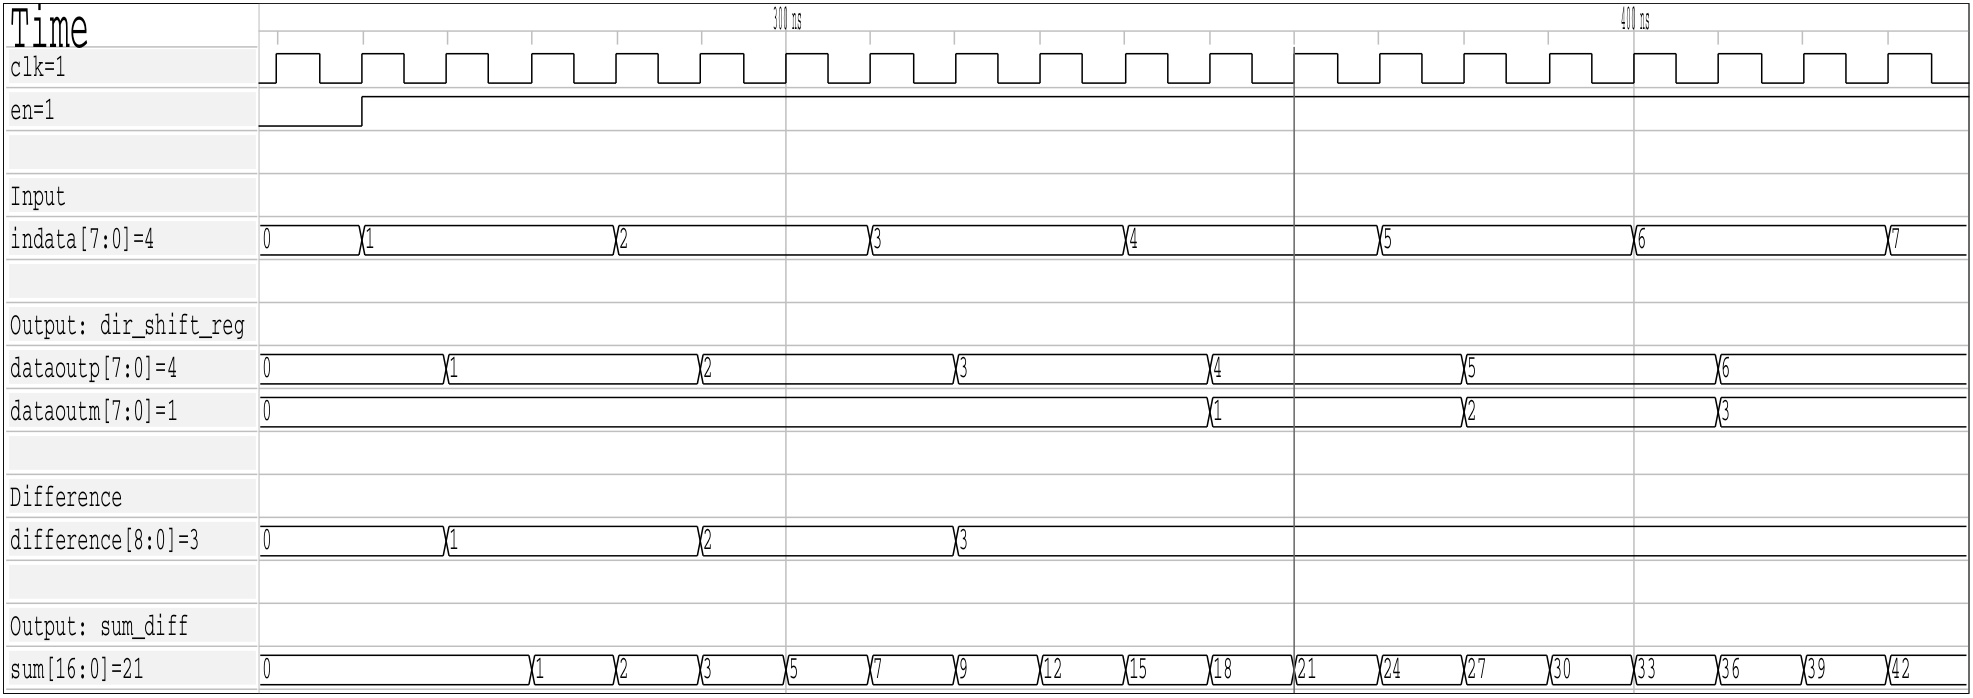
\includegraphics[width=\textwidth]
    {images/image_processing/dir_shift_sum_diff.png}
    \caption{Simulation of the \texttt{dir\_shift\_reg} and the
    \texttt{sum\_diff} block with a \texttt{WIN\_SIZE} of 9}
    \label{fig:sim_shift_sum}
\end{figure}


\subsubsection*{Wallis Algorithm}
Block diagram \ref{fig:wallis_vhdl} is based on the equations of the Wallis algorithm \ref{eq:wallis_filter}.
The pixel to be calculated is connected to the IP core via AXI4-Stream. The constant parameters are connected to the \texttt{controller} and sent from the computer. \\
The division is implemented using the \texttt{Divider Generator}. This is an IP
core
by Xilinx that can be configuered to implement different algorithms for
divisions. Once the pixel is calculated, it is sent to the controller via AXI4-Stream.

\begin{figure}[tb!]
    \centering
    \begin{adjustbox}{max width=\textwidth}
        % \tikzsetnextfilename{system-overview}

\tikzset{%
  do path picture/.style={%
    path picture={%
      \pgfpointdiff{\pgfpointanchor{path picture bounding box}{south west}}%
        {\pgfpointanchor{path picture bounding box}{north east}}%
      \pgfgetlastxy\x\y%
      \tikzset{x=\x/2,y=\y/2}%
      #1
    }
  },
  sin wave/.style={do path picture={    
    \draw [line cap=round] (-3/4,0)
      sin (-3/8,1/2) cos (0,0) sin (3/8,-1/2) cos (3/4,0);
  }},
  cross/.style={do path picture={    
    \draw [line cap=round] (-1,-1) -- (1,1) (-1,1) -- (1,-1);
  }},
  plus/.style={do path picture={    
    \draw [line cap=round] (-3/4,0) -- (3/4,0) (0,-3/4) -- (0,3/4);
  }}
}

\begin{tikzpicture}[
    rounded corners=0mm,
    entity/.style={
        draw,
        minimum height=3.5cm,
        minimum width=5.75cm,
        fill=white,
        anchor=north west,
    },
    entity_c/.style={
        circle,
        draw,
        minimum height=1.0cm,
        minimum width=1cm,
        fill=white,
        anchor=north west,
    },
]
    %coordinates
    \coordinate (c_num)         at (0,0);
    \coordinate (c_den)         at (0,-4.5);
    \coordinate (c_add)         at (0,-9);
    \coordinate (c_div)         at (9,0);
    \coordinate (c_plus_num)    at (1.5,-0.5);
    \coordinate (c_plus_den)    at (3.5,-5);
    \coordinate (c_plus_add)    at (3.5,-9.5);
    \coordinate (c_plus)        at (17,-1.39);
    \coordinate (c_cross_num)   at (3.5,-0.5);
    \coordinate (c_cross_den)   at (1.5,-5);
    \coordinate (c_cross_add)   at (1.5,-9.5);

    %nodes

    \begin{pgfonlayer}{main}
        % entities
        \node[entity, label={numerator}] (num) at (c_num) {};
        \node[entity_c, plus] (plus_num) at (c_plus_num) {};
        \node[entity_c, cross] (cross_num) at (c_cross_num) {};
        
        \node[entity, label={denumerator}] (den) at (c_den) {};  
        \node[entity_c, plus] (plus_den) at (c_plus_den) {};
        \node[entity_c, cross] (cross_den) at (c_cross_den) {};
        
        \node[entity, label={addition}] (add) at (c_add) {};
        \node[entity_c, plus] (plus_add) at (c_plus_add) {};
        \node[entity_c, cross] (cross_add) at (c_cross_add) {};
        
        \node[entity, label={Divider Generator}] (div) at (c_div) {LogiCORE IP};
        \node[entity_c, plus] (plus) at (c_plus) {};
        
        
        % ports
        \path[draw,-{Latex[length=2.5mm]}] (-2,-0.86) node[anchor=west,xshift=-0.1cm,yshift=0.3cm]{$I(x,y)$} --  (plus_num.180);
        \path[draw,-{Latex[length=2.5mm]}] (-2,-1.73) node[anchor=west,xshift=-0.1cm,yshift=0.3cm]{$\mu_n$} -|  node[above,xshift=-0.25cm,yshift=0cm] {$-$} (plus_num.270);
        \path[draw,-{Latex[length=2.5mm]}] (-2,-2.6) node[anchor=west,xshift=-0.1cm,yshift=0.3cm]{$c \cdot \sigma_{g}^{2}$} -|  (cross_num.270);

        \path[draw,-{Latex[length=2.5mm]}] (-2,-5.36) node[anchor=west,xshift=-0.1cm,yshift=0.3cm]{$\sigma_{n}^{2}$} --  (cross_den.180);
        \path[draw,-{Latex[length=2.5mm]}] (-2,-6.23) node[anchor=west,xshift=-0.1cm,yshift=0.3cm]{$c$} -| (cross_den.270);
        \path[draw,-{Latex[length=2.5mm]}] (-2,-7.1) node[anchor=west,xshift=-0.1cm,yshift=0.3cm]{$(1-c) \sigma_{g}^{2}$} -|  (plus_den.270);

        \path[draw,-{Latex[length=2.5mm]}] (-2,-9.86) node[anchor=west,xshift=-0.1cm,yshift=0.3cm]{$\mu_n$} --  (cross_add.180);
        \path[draw,-{Latex[length=2.5mm]}] (-2,-10.73) node[anchor=west,xshift=-0.1cm,yshift=0.3cm]{$1-b$} -|  (cross_add.270);
        \path[draw,-{Latex[length=2.5mm]}] (-2,-11.6) node[anchor=west,xshift=-0.1cm,yshift=0.3cm]{$b \cdot \mu_g$} -|  (plus_add.270);

        \path[draw,-{Latex[length=2.5mm]}] (plus.0) -- node[anchor=west,xshift=-0.6cm,yshift=0.3cm]{$I'(x,y)$} (20,-1.75)   ;


        % Interconnects
        \path[draw,-{Latex[length=2.5mm]}] (plus_num.0) -- (cross_num.180);
        \path[draw,-{Latex[length=2.5mm]}] (cross_den.0) -- (plus_den.180);
        \path[draw,-{Latex[length=2.5mm]}] (cross_add.0) -- (plus_add.180);

        \path[draw,-{Latex[length=2.5mm]}] (cross_num.0) -- (div.163);
        \path[draw,-{Latex[length=2.5mm]}] (plus_den.0) -| ++(3,2.72) -- (div.197);
        \path[draw,-{Latex[length=2.5mm]}] (div.0) -- (plus.180);
        \path[draw,-{Latex[length=2.5mm]}] (plus_add.0) -| (plus.270);

        %points


        % Mean and Variance Block
        \begin{pgfonlayer}{foreground}
            \node [draw, fill=gray!20, inner sep=10, fit={($(num.north)+(0,8pt)$) (den) (add) (plus)}, label=Wallis Filter] (wf) {};
        \end{pgfonlayer}

        % Board box
        % \begin{pgfonlayer}{background}
        %     \node [draw, fill=gray!40, inner sep=10, fit={(plus_num) (cross_num)}, label=numerator] (tx) {};
        % \end{pgfonlayer} 



    \end{pgfonlayer}

\end{tikzpicture}
    \end{adjustbox}
    \caption{Concept of the Wallis filter implementation in VHDL}
    \label{fig:wallis_vhdl}
\end{figure}

\subsection{Hurdles} \label{ch:ip:hurdles_vhdl}
This chapter is about the hurdles in programming with VHDL and the
implementation of the mean and the variance value calculation, as well as the
Wallis algorithm.
The division and the storage of fractional numbers are discussed.

\subsubsection*{Mean and variance value calculation}
A division exists in the calculation of the mean and the variance. As already mentioned in chapter \ref{ch:hls:div}, a division on an FPGA is a complex task.
This division is relatively easy to solve. As can be seen from the equation of
the two calculations (\ref{eq:mean} and \ref{eq:var}), the divisor is constant.
This gives the possibility to calculate $1/N$ in advance and to store the
obtained value as a constant on the FPGA. The result consinsts of a multiplication with
two integers on the FPGA that are interpreted as fractionals and can be
calculated in one clock cycle. \\
Calculated $1/441$ results in $\approx 0.00226757$. This number is converted to
binary and results in $\approx 0.00000000100101001001101$. The following number
is stored as a constant $100101001001101$. Note that 8 decimal digits have been
removed. This must be observed in the following calculations, because the
decimal place can change with each calculation. Figure \ref{fig:data_mean_var}
lists the data widths for the calculation of the mean and the variance. The
square brackets contain the entire data width. If there are two numbers in the
square brackets, the first is the entire data width and the second is the
integer width. The sign is in front of the brackets: u for unsigned and s for
signed.

\begin{figure}[tb!]
    \centering
    \begin{adjustbox}{max width=\textwidth, keepaspectratio}
        % \tikzsetnextfilename{system-overview}

\tikzset{%
  do path picture/.style={%
    path picture={%
      \pgfpointdiff{\pgfpointanchor{path picture bounding box}{south west}}%
        {\pgfpointanchor{path picture bounding box}{north east}}%
      \pgfgetlastxy\x\y%
      \tikzset{x=\x/2,y=\y/2}%
      #1
    }
  },
  sin wave/.style={do path picture={    
    \draw [line cap=round] (-3/4,0)
      sin (-3/8,1/2) cos (0,0) sin (3/8,-1/2) cos (3/4,0);
  }},
  cross/.style={do path picture={    
    \draw [line cap=round] (-1,-1) -- (1,1) (-1,1) -- (1,-1);
  }},
  plus/.style={do path picture={    
    \draw [line cap=round] (-3/4,0) -- (3/4,0) (0,-3/4) -- (0,3/4);
  }}
}

\begin{tikzpicture}[
    rounded corners=0mm,
    entity/.style={
        draw,
        minimum height=1.0cm,
        minimum width=3cm,
        fill=white,
        anchor=north west,
    },
    entity_c/.style={
        circle,
        draw,
        minimum height=1.0cm,
        minimum width=1cm,
        fill=white,
        anchor=north west,
    },
]
    %coordinates
    \coordinate (c_shift)      at (0,0);
    \coordinate (c_sum0)        at (7,0);
    \coordinate (c_sum1)        at (7,-3);
    \coordinate (c_plus)        at (12.5,-3.15);
    \coordinate (c_square0)     at (4,-1.5);
    \coordinate (c_square1)     at (5.5,-1.5);
    \coordinate (c_square2)     at (12.5,-1.5);
    \coordinate (c_divide0)     at (11,-0.15);
    \coordinate (c_divide1)     at (11,-3.15);
    \coordinate (c_fifo)        at (1.0,-0.5);

    %nodes

    \begin{pgfonlayer}{main}
        % entities
        \node[entity, label={dir\_shift\_reg}] (shift) at (c_shift) {};
        \node[entity, label={sum\_diff}] (sum0) at (c_sum0) {\huge $\Sigma$};
        \node[entity, label={sum\_diff}] (sum1) at (c_sum1) {\huge $\Sigma$};

        \node[entity_c] (square0) at (c_square0) {$()^2$};
        \node[entity_c] (square1) at (c_square1) {$()^2$};
        \node[entity_c] (square2) at (c_square2) {$()^2$};

        \node[entity_c] (divide0) at (c_divide0) {$\frac{1}{N}$};
        \node[entity_c] (divide1) at (c_divide1) {$\frac{1}{N}$};

        \node [entity_c, plus] (plus) at (c_plus) {};
        \node [draw, fill=white, minimum width=0.5cm, minimum height=0.2cm, anchor=north west, align=center] (fifo) at (c_fifo) {\small FiFo};


        % ports
        \path[draw,-{Latex[length=2.5mm]}] (-2,-0.51) node[above,xshift=0.8cm,yshift=-0.1cm]{pixel \footnotesize$u[8]$} -- (shift.180);
        \path[draw,-{Latex[length=2.5mm]}] (divide0) -- node[above,xshift=0.75cm,yshift=-0.1cm]{$\mu_n$ \footnotesize$u[8]$} (15.2,-0.51);
        \path[draw,-{Latex[length=2.5mm]}] (plus) -- node[above,xshift=0.09cm,yshift=-0.09cm]{$\sigma_{n}^{2}$ \footnotesize$u[14]$} (15.2,-3.51);

        % Interconnects
        \path[draw,-{Latex[length=2.5mm]}] (shift.180) -| ++(0.5,0.15) -- ($(shift.0) + (0,1/6)$);
        \path[draw,-{Latex[length=2.5mm]}] (shift.180) -| ++(0.5,-0.225) -- (fifo.180);
        \path[draw,-{Latex[length=2.5mm]}] (fifo.0) -| ++(0.4,0.06) -- ($(shift.0) + (0,-1/6)$);
        \path[draw,-{Latex[length=2.5mm]}] ($(shift.0) + (0,1/6)$) node[anchor=west,xshift=0cm,yshift=0.19cm] {plus \footnotesize$u[8]$} -- ($(sum0.180) + (0,1/6)$);
        \path[draw,-{Latex[length=2.5mm]}] ($(shift.0) + (0,-1/6)$) node[anchor=west,xshift=0cm,yshift=0.18cm] {minus \footnotesize$u[8]$} -- ($(sum0.180) + (0,-1/6)$);

        \path[draw,-{Latex[length=2.5mm]}] ($(shift.0) + (0,1/6)$) -| (square1.90);
        \path[draw,-{Latex[length=2.5mm]}] ($(shift.0) + (0,-1/6)$) -| (square0.90);


        \path[draw,-{Latex[length=2.5mm]}] (square1.270) node[anchor=west,xshift=0cm,yshift=-0.2cm] {\footnotesize$u[16]$} |- ($(sum1.180) + (0,1/6)$);
        \path[draw,-{Latex[length=2.5mm]}] (square0.270) node[anchor=west,xshift=0cm,yshift=-0.2cm] {\footnotesize$u[16]$} |- ($(sum1.180) + (0,-1/6)$);

        \path[draw,-{Latex[length=2.5mm]}] (sum0.0) node[anchor=west,xshift=0cm,yshift=0.2cm] {\footnotesize$s[17]$} -- (divide0.180);
        \path[draw,-{Latex[length=2.5mm]}] (sum1.0) node[anchor=west,xshift=0cm,yshift=0.2cm] {\footnotesize$s[25]$} -- (divide1.180);

        \path[draw,-{Latex[length=2.5mm]}] (divide1.0) node[above,xshift=0.2cm,yshift=-0.9cm]{\footnotesize$s[40,25]$} -- (plus.181);
        \path[draw,-{Latex[length=2.5mm]}] (divide0.0) node[above,xshift=0.6cm,yshift=-0.1cm]{\footnotesize$s[32,17]$} -| node[above,xshift=-0.6cm,yshift=-0.8cm]{\footnotesize$u[12,8]$} (square2.90);
        \path[draw,-{Latex[length=2.5mm]}] (square2.270) node[above,xshift=-0.6cm,yshift=-0.5cm]{\footnotesize$u[24,16]$} -| node[above,xshift=-0.25cm,yshift=-0.71cm] {$-$} (plus.90);

        %points
        \node[circle, draw=black, fill=black, inner sep=0pt,minimum size=1.6pt] (b) at (0.5,-0.509) {};
        \node[circle, draw=black, fill=black, inner sep=0pt,minimum size=1.6pt] (b) at (4.359,-0.674) {};
        \node[circle, draw=black, fill=black, inner sep=0pt,minimum size=1.6pt] (b) at (5.859,-0.344) {};
        \node[circle, draw=black, fill=black, inner sep=0pt,minimum size=1.6pt] (b) at (12.859,-0.509) {};

        % Mean and Variance Block
        \begin{pgfonlayer}{foreground}
            \node [draw, fill=gray!20, inner sep=10, fit={(shift) ($(shift.north)+(0,8pt)$) (sum0) (sum1) (plus) (square0) (square1) (square2) (divide0) (divide1)}, label=Mean \& Variance] (mv) {};
        \end{pgfonlayer}



    \end{pgfonlayer}

\end{tikzpicture}
    \end{adjustbox}
    \caption{Data width of mean and variance calculation}
    \label{fig:data_mean_var}
\end{figure}

\subsubsection*{Wallis Algorithm}
The Wallis algorithm also contains a division. In this case, however, it is not
possible to simplify it
because the numerator and denumerator change with each pixel. \\
Xilinx offers an IP core which solves divisions. It is called \texttt{Divider
Generator} \cite{divider}. The \texttt{Divider Generator} contains three different implementations of divisions (LUTMult, Radix-2, High Radix). These three divisions are distinguished by resource consumption, latency and throughput. The numerator and denumerator can be passed to the \texttt{Divider Generator} via AXI4-Stream. The result is again sent via AXI4-Stream. \\
The decision was made to implement the High-Radix algorithm. Due to the size of
the dividend the LUTMult was omitted and because of the latency the implementation of the Radix-2. The divider should accept a new division after at most 21 clock cycles, because this is the time of the iteration sequence. This is fulfilled by the implementation of the High-Radix. The latency and throughput of the calculation can be influenced during implementation \cite{divider}.
